\begin{figure}[tb]
\centering
\begin{tikzpicture}[
  x=1cm,y=1cm,
  axis/.style={circle,draw,fill=white,inner sep=1.6pt},
  root/.style={line width=.7pt},
  newroot/.style={line width=1.2pt,blue!60!black},
  every node/.style={font=\small}]
  \node[axis] (p0) at (0,0) {};
  \node[axis] (p1) at (1.3,.85) {};
  \node[axis] (p2) at (1.3,-.85) {};
  \node[axis] (q0) at (4.3,0) {};
  \node[axis] (q1) at (5.6,.85) {};
  \node[axis] (q2) at (5.6,-.85) {};
  \draw[root] (p0)--(p1)--(p2);
  \draw[root,dashed] (p2)--(p0);
  \draw[root] (q0)--(q1)--(q2);
  \draw[root,dashed] (q2)--(q0);
  \draw[newroot] (p1)--node[above,sloped] {new joining root}
    node[below,sloped] {$|d_e|=1$} (q0);
  \node at (.65,1.45) {$P$: odd assigned parity};
  \node at (4.95,1.45) {$Q$: odd assigned parity};
  \node[align=center] at (.65,-1.5)
    {cycle: $m_e^0\in\Z+\tfrac12$\\$|d_e|=\tfrac12$};
  \node[align=center] at (4.95,-1.5)
    {cycle: $m_e^0\in\Z+\tfrac12$\\$|d_e|=\tfrac12$};
  \draw[root] (0,-2.3)--(.5,-2.3);
  \node[anchor=west] at (.6,-2.3) {equal-sign identification};
  \draw[root,dashed] (0,-2.8)--(.5,-2.8);
  \node[anchor=west] at (.6,-2.8) {opposite-sign identification};
\end{tikzpicture}
\caption{The graph underlying the half-relation deformation.
The two original components are unbalanced and have odd assigned
difference parity. A joining root connects their even-sum lattices
inside the full type-$D$ root lattice. For the displayed graph,
half the primitive relation has absolute value $\tfrac12$ on the
cycles and $1$ on the joining edge. More generally the latter
value occurs on the whole connecting path, and coefficients on
other attached trees vanish. Cycle lengths and omitted branches
are schematic; local feasibility is supplied by a local link.}
\label{fig:half-relation}
\end{figure}
